
	It has been said that all maths is graph theory.
	
	This is a slight exaggeration. However, graph theory has proven to be an extremely useful branch of mathematics for computer science (in which it is used for modelling social media, travel (e.g. GPS algorithms), computer chip design, and a multitude of other areas), linguistics (in modelling of natural language syntax and word meaning), chemistry, physics, neuroscience, sociology, wildlife conservation, and even urban planning \cite{acityisnotatree}, to name but a few.

	\paragraph{Graphs}
	
	Unsurprisingly, graph theory is the study of \textit{graphs}, which bear no relation to bar charts and other statistical diagrams. The most basic kind of graph (a \textit{simple}, \textit{undirected} graph) is defined rigorously as an ordered pair \(G=(V,E)\), where \(V\) is a set of \textit{vertices} and \(E\) a set of \textit{edges}, each of which is a subset of \(V\) containing two elements. This is really just a way of representing a collection of points (which we call vertices (or sometimes points or nodes)) with lines (which we call edges (or sometimes arcs or lines)) drawn between some of them.
	
	\begin{figure}[h]
		\centering
		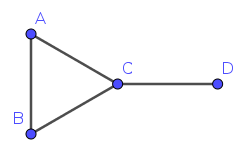
\includegraphics[width=0.5\textwidth]{simplegraph}
		\caption{A simple, undirected graph}
		\label{simplegraph}
	\end{figure}
	
	Figure \ref{simplegraph} would have \(V={A,B,C,D}\), as these are the vertices of the graph, and \(E=\{\{A,B\},\{A,C\},\{B,C\},\{C,D\}\}\), as each of the pairs represents one edge on the graph. We say that a graph is \textit{undirected} if it is not \textit{directed}\footnote{This term will be defined later.\label{definedlater}}.
	
	We say a graph is \textit{simple} if there are no edges which go from one vertex back to the same vertex (such edges are called \textit{loops}) and at most one edge goes between any pair of vertices. Graphs that are not necessarily simple are sometimes called \textit{multigraphs}, \textit{pseudographs}, or \textit{general graphs}, but this term is rather poorly defined, as there is no consensus as to whether these terms allow loops, among other issues; if one uses these terms, one ought to define its meaning before doing so. There is also confusion as to whether \textit{graphs} are by default simple or not; one ought to specify this when this distinction is of any importance.
	
	A graph \(G\)'s \textit{vertex set} (the set of vertices) is notated \(V(G)\), and similarly its \textit{edge set} \(E(G)\). We often abbreviate an edge \(\{A,B\}\) to just \(AB\).
	
	\paragraph{Digraphs}
	
	Digraphs are \textit{directed graphs} (hence the name \textit{digraph}); their primary characteristic that sets them apart from other graphs is that the edges have a direction, thus:
	
	\begin{figure}[h]
		\centering
		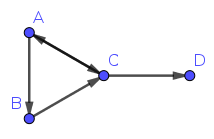
\includegraphics[width=0.5\textwidth]{directedgraph}
		\caption{A directed graph}
		\label{directedgraph}
	\end{figure}
	
	A digraph is defined rigorously as an ordered pair \(G=(V,E)\), where \(V\) is a set of \textit{vertices} and \(E\) a set of \textit{edges}, just as a normal graph; however, \(E\) instead contains ordered pairs, so that a pair \((X,Y)\) indicates that there is an edge from \(X\) to \(Y\). In Figure \ref{directedgraph}, \(V={A,B,C,D}\) and \(E=\{(A,B),(A,C),(B,C),(C,A),(C,D)\}\). Note that this digraph is still considered simple, as while we have two edges between \(A\) and \(C\), they are in different directions.
	
	Unless otherwise stated, the word \textit{graph} does not usually include digraphs.
	
	\paragraph{Walks}
	
	Much of graph theory concerns itself with \textit{walks} between vertices. A walk from vertex \(X\) to vertex \(Y\) is essentially a way to go from from \(X\) to \(Y\) \say{walking} only along edges; on digraphs, one must \say{walk} in the direction of an edge. For example, in Figure \ref{simplegraph}, \(B \rightarrow A \rightarrow C \rightarrow D\) is a walk from \(B\) to \(D\); however, this is not a valid walk on the directed graph in Figure \ref{directedgraph}, as there is no edge from \(B\) to \(A\). Instead, one must take the walk \(B \rightarrow C \rightarrow D\).
	
	\textit{Paths} are walks where each vertex occurs at most once in the walk. \textit{Trails} are walks which do not go over any edges more than once. \textit{Cycles} are walks that go from a vertex back to itself (they are considered to visit this vertex only once).
	
	A \textit{Hamiltonian path} on a given graph is a path that goes through every vertex exactly once, and \textit{Hamiltonian cycles} are cycles that visit every vertex exactly once. Graphs with Hamiltonian paths are called \textit{Hamiltonian graphs}.
	
	An \textit{Eulerian trail} (or sometimes \textit{Eulerian path}, although this is a misuse of the term path) is a trail that goes through every edge exactly once, and similarly an \textit{Eulerian cycle} is an Eulerian trail that is also a cycle. \textit{Eulerian graphs}, somewhat predictably, are graphs with Eulerian trails.
	
	In fact, the first ever graph theory theorem was about \textit{Eulerian paths}. The famous mathematician Leonhard Euler wanted to know if there was a way to walk through the Prussian city of K\"onigsberg (now Kaliningrad in Russia) and cross each of its seven bridges exactly once (without crossing the river by any other means). K\"onigsberg had two large islands, and the bridges were situated as in Figure \ref{Konigsberg}.
	
	\begin{figure}[h]
		\centering
		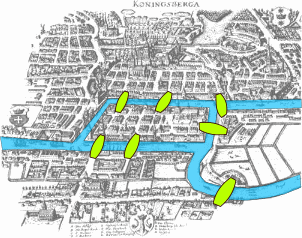
\includegraphics[width=0.5\textwidth]{Konigsberg}
		\caption{The Seven Bridges of K\"onigsberg, as they were in Euler's time}
		\label{Konigsberg}
	\end{figure}
	
	We can consider this as a graph (shown in Figure \ref{Konigsberggraph}), with the vertices being the land masses and the edges being the bridges; then Euler's walk across all the bridges is an Eulerian trail on our graph.
	
	\begin{figure}[h]
		\centering
		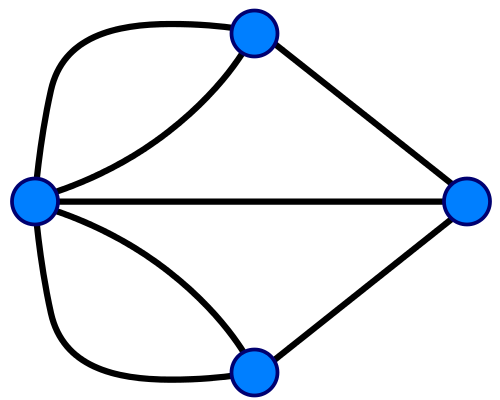
\includegraphics[width=0.5\textwidth]{Konigsberggraph}
		\caption{A graph theoretic representation of the Seven Bridges}
		\label{Konigsberggraph}
	\end{figure}
	
	Except for the first and last times we cross an edge/bridge, whenever we enter a vertex/land mass, we then leave it. This means that all vertices/land masses except those at the ends of our trail must be entered as many times as they are left, and so must have even degree.
	
	If we start and end at different vertices/land masses, they must have odd degree, as we leave the former one more time than we enter it, and enter the latter one more time than we leave it. If we start and end at the same vertex/land mass, it has even degree, as we enter it as many times as we leave it.
	
	However, the graph of K\"onigsberg has four vertices, all of which have odd degree. Thus we cannot find an Eulerian trail, as at most two vertices can have odd degree for an Eulerian trail to exist.
	
	It was stated by Euler, and later proven by Carl Hierholzer just before his death in 1871, that we can find an Eulerian trail if and only if there are exactly zero or two vertices of odd degree in a graph, and the graph is \textit{connected}. (A graph is said to be connected if there is a walk between any two vertices. Figure \ref{simplegraph} shows a connected graph, while Figure \ref{disconnectedgraph} does not.)
	
	\begin{figure}[h]
		\centering
		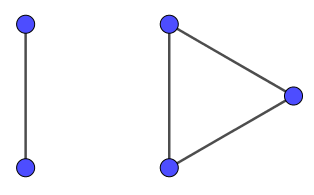
\includegraphics[width=0.5\textwidth]{disconnectedgraph}
		\caption{A disconnected graph}
		\label{disconnectedgraph}
	\end{figure}
	
	\paragraph{Trees}
	
	\textit{Trees} are graphs where there is exactly one path between any two vertices, as in Figure \ref{treegraph}. An equivalent definition is that trees are graphs that are both \textit{acyclic} (having no cycles) and connected.
	
	\begin{figure}[h]
		\centering
		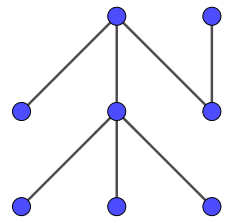
\includegraphics[width=0.5\textwidth]{treegraph}
		\caption{A tree.}
		\label{treegraph}
	\end{figure}
	
	A \textit{forest} is a \textit{disjoint union} (in graph theory, this essentially means \say{the graph you get by putting several graphs next to each other without adding any new edges}) of several trees.
	
	Every tree or forest is bipartite\footnotemark[\ref{definedlater}], and every \textit{finite} (having finitely many vertices) tree or forest is planar\footnotemark[\ref{definedlater}].
	
	\paragraph{Bipartite Graphs}
	
	Bipartite graphs are graphs where the vertex set (the set of vertices) of the graph can be divided into two \textit{disjoint} (having no elements in common) sets \(T,U\) so that there are no edges between two vertices in \(T\), and no edges between two vertices in \(U\). It follows that all edges are between vertices in different sets.
	
	An equivalent definition is that graphs are bipartite if and only if they do not contain any \textit{odd cycles} (cycles with an odd number of vertices). One can see why this should be true, as we can divide any single \textit{even cycle} into two sets \(T,U\) to fit our condition by simply alternating which set we put points in as we go round the cycle. It is a little more complex to prove.
	
	It follows that all trees are bipartite, and Figure \ref{bipartitetree} shows the graph from Figure \ref{treegraph} divided into sets \(T,U\), with vertices moved to indicate this.
	
	\begin{figure}[h]
		\centering
		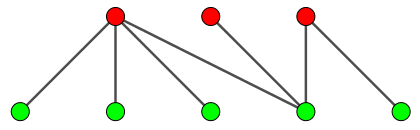
\includegraphics[width=0.5\textwidth]{bipartitetree}
		\caption{The tree shown in Figure \ref{treegraph} divided into two sets so as to prove it to be bipartite.}
		\label{bipartitetree}
	\end{figure}
	
	Another equivalent definition is that a graph is bipartite if and only if it is \textit{2-colorable}\footnotemark[\ref{definedlater}].
	
	\paragraph{Complete Graphs}
	
	The \textit{complete graph} \(K_n\) is the graph with \(n\) vertices where there is an edge between every two vertices. Figure \ref{k5graph} shows \(K_5\), the complete graph vertices.
	
	\begin{figure}[h]
		\centering
		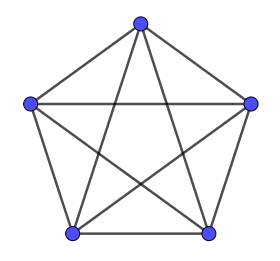
\includegraphics[width=0.5\textwidth]{k5graph}
		\caption{\(K_5\)}
		\label{k5graph}
	\end{figure}
	
	The \textit{complete bipartite graph} \(K_{m,n}\) is the bipartite graph where set \(T\) has \(m\) vertices, set \(U\) has \(n\) vertices, and there is an edge from every vertex in \(T\) to every vertex in \(U\). Figure \ref{utilitygraph} shows \(K_{3,3}\), which is also known as the utility graph, after the three utilities problem.
	
	\begin{figure}[h]
		\centering
		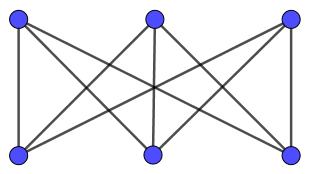
\includegraphics[width=0.5\textwidth]{utilitygraph}
		\caption{\(K_{3,3}\)}
		\label{utilitygraph}
	\end{figure}
	
	\paragraph{Planar Graphs}
	
	The three utilities problem is stated thus:
	
	\begin{displayquote}
		Suppose there are three cottages on a plane (or sphere) and each needs to be connected to the gas, water, and electricity companies. Without using a third dimension or sending any of the connections through another company or cottage, is there a way to make all nine connections without any of the lines crossing each other?
	\end{displayquote}
	
	This turns out not to be possible. This is really a graph theory question, and can be phrased more succinctly thus:
	
	\begin{displayquote}
		Is \(K_{3,3}\) a planar graph?
	\end{displayquote}
	
	A \textit{planar graph} is a graph that can be drawn on a plane (e.g. a flat piece of paper) so that none of the edges cross each other.
	
	A \textit{subdivision} of a graph \(G\) is a graph which can be obtained by dividing edges of \(G\) and placing new points in the place where we have divided them; we are thus allowed to turn edges into the configuration shown in Figure \ref{subdivision}. More rigorously, we are saying that we are allowed to turn the edge \(\{A,B\}\), for any vertices \(A,B\), into the two edges \(\{A,C\},\{C,B\}\), where \(C\) is a new vertex we have just introduced. We can do this repeatedly, and turn \(\{A,B\}\) into \(\{A,C\},\{C,D\},\{D,B\}\).
	
	\begin{figure}[h]
		\centering
		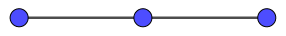
\includegraphics[width=0.5\textwidth]{subdivision}
		\caption{A subdivision of a single edge.}
		\label{subdivision}
	\end{figure}
	
	A \textit{subgraph} of a graph \(G\) is a graph whose vertex set is a subset of that of \(G\), and whose edge set is a subset of that of \(G\). The vertex set of the subgraph must include the endpoints of all the edges of the subgraph, but may also include lone vertices of degree 0.
	
	\textbf{Kuratowski's theorem} states a graph is planar if and only if it does not contain a subgraph that is a subdivision of \(K_5\) or \(K_{3,3}\). This theorem was independently proven by Kazimierz Kuratowski, Orrin Frink, and Paul Smith in 1930. Karl Menger also proved it on graphs where all vertices have degree 3 in 1930.
	
	\paragraph{Colourings}
	
	\textit{Colourings} are ways to label aspects of a graph with colours subject to certain constraints. The two most common types of colourings are vertex colourings, where we colour vertices such that no two vertices with an edge between them are of the same colour, and edge colourings, where we colour edges so that no two edges with an endpoint in common have the same colour. You have probably encountered graph colouring before in Sudoku, which is really a question of colouring an graph with 81 vertices with 9 colours.
	
	The \textit{chromatic number} of a graph is the smallest number of colours required to colour a graph's vertices. We say a graph is \textit{\(n\)-colourable} if its vertices can be coloured with \(\leq{}n\) colours.
	
	The \textbf{four colour theorem} states that any planar graph can be 4-coloured (although it is usually phrased in terms of maps, which, assuming no two separate regions are forced to be the same colour, can be 4-coloured; in fact, map colourings and planar graph colourings are isomorphic).
	
	It was proved in 1976 by Kenneth Appel and Wolfgang Haken, and was the first major theorem proved using a computer. However, the five colour theorem (which says that all planar graphs are 5-colourable) was proved in 1980.
	
	\subsection{Problems}
	
	\begin{enumerate}
		\item Prove the five colour theorem.
		\item A polyhedral graph is a connected graph where the vertices and edges are those of a convex polyhedron (or, equivalently, the removal of any two vertices does not render the graph disconnected). A bicubic graph is both bipartite and cubic. A cubic graph is a graph where all vertices have degree 3. Do all bicubic polyhedral graphs have Hamiltonian cycles?
	\end{enumerate}
		
	\begin{thebibliography}{9}
		\bibitem{acityisnotatree}
		Christopher Alexander,
		\textit{A City is Not a Tree},
		1965.
	\end{thebibliography}
	